%%%%%%%%%%%%%%%%%%%%%%%%%%%%%%%%%%%%%%%%%
% Arsclassica Article
% LaTeX Template
% Version 1.1 (1/8/17)
%
% This template has been downloaded from:
% http://www.LaTeXTemplates.com
%
% Original author:
% Lorenzo Pantieri (http://www.lorenzopantieri.net) with extensive modifications by:
% Vel (vel@latextemplates.com)
%
% License:
% CC BY-NC-SA 3.0 (http://creativecommons.org/licenses/by-nc-sa/3.0/)
%
%%%%%%%%%%%%%%%%%%%%%%%%%%%%%%%%%%%%%%%%%

%----------------------------------------------------------------------------------------
%	PACKAGES AND OTHER DOCUMENT CONFIGURATIONS
%----------------------------------------------------------------------------------------

\documentclass[
10pt, % Main document font size
a4paper, % Paper type, use 'letterpaper' for US Letter paper
oneside, % One page layout (no page indentation)
%twoside, % Two page layout (page indentation for binding and different headers)
headinclude,footinclude, % Extra spacing for the header and footer
BCOR5mm, % Binding correction
table,
]{scrartcl}

%%%%%%%%%%%%%%%%%%%%%%%%%%%%%%%%%%%%%%%%%
% Arsclassica Article
% Structure Specification File
%
% This file has been downloaded from:
% http://www.LaTeXTemplates.com
%
% Original author:
% Lorenzo Pantieri (http://www.lorenzopantieri.net) with extensive modifications by:
% Vel (vel@latextemplates.com)
%
% License:
% CC BY-NC-SA 3.0 (http://creativecommons.org/licenses/by-nc-sa/3.0/)
%
%%%%%%%%%%%%%%%%%%%%%%%%%%%%%%%%%%%%%%%%%

%----------------------------------------------------------------------------------------
%	REQUIRED PACKAGES
%----------------------------------------------------------------------------------------

\usepackage[
nochapters, % Turn off chapters since this is an article        
beramono, % Use the Bera Mono font for monospaced text (\texttt)
eulermath,% Use the Euler font for mathematics
pdfspacing, % Makes use of pdftex’ letter spacing capabilities via the microtype package
dottedtoc % Dotted lines leading to the page numbers in the table of contents
]{classicthesis} % The layout is based on the Classic Thesis style



\usepackage[hmarginratio=1:1,top=25mm,left=20mm,columnsep=25pt]{geometry}
\usepackage{relsize} % e.g. used for \mathsmaller
\usepackage{bm}

\usepackage{arsclassica} % Modifies the Classic Thesis package

\usepackage[T1]{fontenc} % Use 8-bit encoding that has 256 glyphs

\usepackage[utf8]{inputenc} % Required for including letters with accents

\usepackage{graphicx} % Required for including images
\graphicspath{{Figures/}} % Set the default folder for images

\usepackage{enumitem} % Required for manipulating the whitespace between and within lists

\usepackage{lipsum} % Used for inserting dummy 'Lorem ipsum' text into the template

\usepackage{subfig} % Required for creating figures with multiple parts (subfigures)

\usepackage{amsmath,amssymb,amsthm} % For including math equations, theorems, symbols, etc

\usepackage{varioref} % More descriptive referencing

\usepackage{accents}

\usepackage[bottom]{footmisc}

\usepackage{titling} % it needs to define \thanksmarkseries

%----------------------------------------------------------------------------------------
% NEW COMMANDS
%----------------------------------------------------------------------------------------
\renewcommand{\AA}{\bm{A}}
\newcommand{\GG}{\bm{G}}
\newcommand{\MM}{\bm{M}}
\newcommand{\Id}{\bm{I}}
\newcommand{\vv}{\bm{v}}
\newcommand{\QQ}{\bm{Q}}
\renewcommand{\SS}{\bm{S}}
\newcommand{\Lie}{\mathfrak{L}}
\newcommand{\calE}{\mathcal{E}}						%

\newcommand{\IP}[1]{{\color{Red}IP:\ \ #1}}
\newcommand{\ER}[1]{{\color{Green}ER:\ \ #1}}
\newcommand{\BL}[1]{{\color{Cerulean}BL:\ \ #1}}
\newcommand{\NF}[1]{{\color{Plum}NF:\ \ #1}}


\newcommand{\sA}{\mathsmaller A}
\newcommand{\sB}{\mathsmaller B}
\newcommand{\sC}{\mathsmaller C}
\newcommand{\sD}{\mathsmaller D}
\newcommand{\sM}{\mathsmaller M}
\newcommand{\sN}{\mathsmaller N}
\newcommand{\sL}{\mathsmaller L}
\newcommand{\kronecker}[2]{\delta^{#1}_{\phantom{#1}#2}}
\newcommand{\durg}[2]{ D_{#1}^{\phantom{#1}#2} }	% Eulerian components of 
%the D field
\newcommand{\LeviCivitaUp}[1]{\varepsilon^{#1}}

\newcommand{\pd}{\partial}
\newcommand{\F}[2]{F^{\ #1}_{\mathsmaller#2}}
\newcommand{\hatF}[2]{\hat{F}^{\ #1}_{\mathsmaller#2}}
\newcommand{\A}[2]{A^{\mathsmaller#1}_{\ #2}}

\newcommand{\dist}[2]{ A^{#1}_{\phantom{#1}#2} }	% Component of the 
\newcommand{\Stress}[2]{ \Sigma^{#1}_{\phantom{#1}#2} }	% Total stress tensor
%distortion field A
\newcommand{\distsmall}[2]{ a_{{#1}{#2}} }	% Small distortion field A 
\newcommand{\Dist}{ \bm{A} }	% Distortion field A in matrix notations
\newcommand{\Burg}{ \bm{B} }	% Burgers tensor = curl(A)
\newcommand{\Durg}{ \bm{D} }	% Complimentary to the Burgers
\newcommand{\Distsmall}{ \bm{a} }	% Small distortion field A in matrix 
%notations
\newcommand{\Plastsmall}{ \bm{\pi} }	% Small distortion field A in matrix 
%notations
\newcommand{\Defgrad}{ \bm{F} }
\newcommand{\iDist}{ \bm{E} }
\newcommand{\symA}{\text{sym}(\bm{a})}
\newcommand{\skewA}{\text{skew}(\bm{a})}
\newcommand{\symP}{\text{sym}(\bm{\Plastsmall})}
\newcommand{\burg}[2]{ B^{{#1}{#2}} }	% Eulerian components of the B field
\newcommand{\itetr}[2]{e^{\phantom{#2}#1}_{#2}}
\newcommand{\tetr}[2]{a^{#1}_{\phantom{#1}#2}}
\newcommand{\rtetr}[2]{a^{#1}_{(\text{r}) #2}}
\newcommand{\spin}[2]{\omega^{#1}_{\phantom{#1}#2}}
\newcommand{\Lor}[2]{\Lambda^{#1'}_{\phantom{#1}#2}}
\newcommand{\iLor}[2]{\Lambda^{\phantom{#2}#1}_{#2'}}
\newcommand{\vel}[1]{v^{#1}}
\newcommand{\D}[1]{\mathcal{D}_{#1}} % Fock-Ivanencko cov derivative
\newcommand{\Tors}[2]{T^{#1}_{\phantom{a}#2}}
\newcommand{\Supp}[2]{S_{#1}^{\phantom{a}#2}}	%supepotential
\newcommand{\Torsl}[1]{T_{#1}}
\newcommand{\ET}[2]{E^{#1}_{\phantom{#1}#2}}	%Torsion decomposition, analog 
%of Electric field
\newcommand{\eT}[2]{D_{#1}^{\phantom{#1}#2}}	%Torsion decomposition, analog 
%of Electric field
\newcommand{\BT}[2]{B^{#1#2}}	%Torsion decomposition, analog of Magnetic field
\newcommand{\hT}[2]{H^{#1#2}}	%Torsion decomposition, analog of Magnetic field
\newcommand{\W}[2]{\mathcal{W}^{#1}_{\phantom{#1}#2}}
\newcommand{\w}[2]{W^{#1}_{\phantom{#1}#2}}
\newcommand{\FI}{Fock-Ivanenko}
\newcommand{\We}{Weitzenb\"ock}
\newcommand{\Lag}{\mathcal{L}}	% Lagrangian which depends on ordinary 
%derivatives
\newcommand{\Lagcov}{\pounds}% Lagrangian which depends on gauge covariant 
%derivatives
\newcommand{\Laghodge}{L}% Lagrangian which depends on the Hodge dual of the 
%torsion
\newcommand{\Lagtors}{\mathbb{L}}% Lagrangian which depends on torsion
\newcommand{\LagBE}{\mathfrak{L}}% Lagrangian which depends on the B and E 
%fields
\newcommand{\veps}{\varepsilon}
\newcommand{\EM}[2]{\Sigma^{#1}_{\phantom{#1}#2}}
\newcommand{\transpose}{{\mathrm {\mathsmaller T}}}
\newcommand{\tr}{\text{tr}}

\newcommand{\tegr}{TEGR}
\newcommand{\HT}[1]{\accentset{\star}{T}^{#1}}

\newcommand{\csh}{c_\text{sh}}	% 	shear sound speed
\newcommand{\csp}{c_\text{sp}}	% 	a sound speed related to the spin
\newcommand{\cinf}{c_\infty}	% 	a sound speed related to 
%1/\sqrt{\mu\eps}
%----------------------------------------------------------------------------------------
%	THEOREM STYLES
%---------------------------------------------------------------------------------------

\theoremstyle{definition} % Define theorem styles here based on the definition style (used for definitions and examples)
\newtheorem{definition}{Definition}

\theoremstyle{plain} % Define theorem styles here based on the plain style (used for theorems, lemmas, propositions)
\newtheorem{theorem}{Theorem}

\theoremstyle{remark} % Define theorem styles here based on the remark style (used for remarks and notes)

%----------------------------------------------------------------------------------------
%	HYPERLINKS
%---------------------------------------------------------------------------------------




%----------------------------------------------------------------------------------------
%	BIBLATEX
%---------------------------------------------------------------------------------------

\usepackage[backend=bibtex,giveninits=true,url=false,doi=true,eprint=true,isbn=false,
backref,backrefstyle=none,maxbibnames=99]{biblatex}
\DefineBibliographyStrings{english}{%
  backrefpage = {Cited on p\adddot},%
  backrefpages = {Cited on pp\adddot}%
}

\bibliography{library}

\renewcommand*{\bibfont}{\footnotesize}

% in order to suppress 'In:'
\renewbibmacro{in:}{%
  \ifboolexpr{%
     test {\ifentrytype{article}}%
  }{}{\printtext{\bibstring{in}\intitlepunct}}%
}

%----------------------------------------------------------------------------------------
% these commands allow to put equations in a fancy boxes:
%----------------------------------------------------------------------------------------
\usepackage{empheq}
\newlength\mytemplen
\newsavebox\mytempbox
\makeatletter
\definecolor{cream}{rgb}{.81, .88, 1}
 \newcommand\mycreambox{%
     \@ifnextchar[%]
        {\@mycreambox}%
        {\@mycreambox[0pt]}}
 \def\@mycreambox[#1]{%
     \@ifnextchar[%]
        {\@@mycreambox[#1]}%
        {\@@mycreambox[#1][0pt]}}
 \def\@@mycreambox[#1][#2]#3{
     \sbox\mytempbox{#3}%
     \mytemplen\ht\mytempbox
     \advance\mytemplen #1\relax
     \ht\mytempbox\mytemplen
     \mytemplen\dp\mytempbox
     \advance\mytemplen #2\relax
     \dp\mytempbox\mytemplen
     \colorbox{cream}{\hspace{1em}\usebox{\mytempbox}\hspace{1em}}}
 \makeatother

% ------------------------------------------------------------------------------
\newcommand*\samethanks[1][\value{footnote}]{\footnotemark[#1]}

 % Include the structure.tex file which specified the document structure and 
%layout

\usepackage[hmarginratio=1:1,top=25mm,left=40mm,columnsep=25pt]{geometry}
\usepackage{hyperref}
\usepackage{relsize} % e.g. used for \mathsmaller
\usepackage{bm}


\newcommand{\Id}{\bm{I}}
\newcommand{\vv}{\bm{v}}
\newcommand{\QQ}{\bm{Q}}
\renewcommand{\SS}{\bm{S}}
\newcommand{\Lie}{\mathfrak{L}}
\newcommand{\calE}{\mathcal{E}}						%

\newcommand{\IP}[1]{{\color{Red}IP:\ \ #1}}


\newcommand{\sA}{\mathsmaller A}
\newcommand{\sB}{\mathsmaller B}
\newcommand{\sC}{\mathsmaller C}
\newcommand{\sD}{\mathsmaller D}
\newcommand{\sM}{\mathsmaller M}
\newcommand{\sN}{\mathsmaller N}
\newcommand{\sL}{\mathsmaller L}

\newcommand{\pd}{\partial}
\newcommand{\F}[2]{F^{\ #1}_{\mathsmaller#2}}
\newcommand{\hatF}[2]{\hat{F}^{\ #1}_{\mathsmaller#2}}
\newcommand{\A}[2]{A^{\mathsmaller#1}_{\ #2}}

\newcommand{\dist}[2]{ A_{{#1}{#2}} }	% Distortion field A
\newcommand{\distsmall}[2]{ a_{{#1}{#2}} }	% Small distortion field A 
\newcommand{\Dist}{ \bm{A} }	% Distortion field A in matrix notations
\newcommand{\Burg}{ \bm{B} }	% Burgers tensor = curl(A)
\newcommand{\Durg}{ \bm{D} }	% Complimentary to the Burgers
\newcommand{\Distsmall}{ \bm{a} }	% Small distortion field A in matrix notations
\newcommand{\Plastsmall}{ \bm{p} }	% Small distortion field A in matrix notations
\newcommand{\Defgrad}{ \bm{F} }
\newcommand{\iDist}{ \bm{E} }
\newcommand{\symA}{\text{sym}(\bm{a})}
\newcommand{\skewA}{\text{skew}(\bm{a})}
\newcommand{\symP}{\text{sym}(\bm{p})}
\newcommand{\burg}[1]{ B_{#1} }	% Burgers
\newcommand{\itetr}[2]{e^{\phantom{#2}#1}_{#2}}
\newcommand{\tetr}[2]{a^{#1}_{\phantom{#1}#2}}
\newcommand{\rtetr}[2]{a^{#1}_{(\text{r}) #2}}
\newcommand{\spin}[2]{\omega^{#1}_{\phantom{#1}#2}}
\newcommand{\Lor}[2]{\Lambda^{#1'}_{\phantom{#1}#2}}
\newcommand{\iLor}[2]{\Lambda^{\phantom{#2}#1}_{#2'}}
\newcommand{\D}[1]{\mathcal{D}_{#1}} % Fock-Ivanencko cov derivative
\newcommand{\Tors}[2]{T^{#1}_{\phantom{a}#2}}
\newcommand{\Supp}[2]{S_{#1}^{\phantom{a}#2}}	%supepotential
\newcommand{\Torsl}[1]{T_{#1}}
\newcommand{\ET}[2]{E^{#1}_{\phantom{#1}#2}}	%Torsion decomposition, analog of Electric field
\newcommand{\eT}[2]{D_{#1}^{\phantom{#1}#2}}	%Torsion decomposition, analog of Electric field
\newcommand{\BT}[2]{B^{#1#2}}	%Torsion decomposition, analog of Magnetic field
\newcommand{\hT}[2]{H^{#1#2}}	%Torsion decomposition, analog of Magnetic field
\newcommand{\W}[2]{\mathcal{W}^{#1}_{\phantom{#1}#2}}
\newcommand{\w}[2]{W^{#1}_{\phantom{#1}#2}}
\newcommand{\FI}{Fock-Ivanenko}
\newcommand{\We}{Weitzenb\"ock}
\newcommand{\Lag}{\mathcal{L}}	% Lagrangian which depends on ordinary derivatives
\newcommand{\Lagcov}{\pounds}% Lagrangian which depends on gauge covariant derivatives
\newcommand{\Laghodge}{L}% Lagrangian which depends on the Hodge dual of the torsion
\newcommand{\Lagtors}{\mathbb{L}}% Lagrangian which depends on torsion
\newcommand{\LagBE}{\mathfrak{L}}% Lagrangian which depends on the B and E fields
\newcommand{\veps}{\varepsilon}
\newcommand{\EM}[2]{\Sigma^{#1}_{\phantom{#1}#2}}
\newcommand{\transpose}{{\mathrm {\mathsmaller T}}}
\newcommand{\tr}{\text{tr}}

\newcommand{\tegr}{TEGR}
\newcommand{\HT}[1]{\accentset{\star}{T}^{#1}}

\hyphenation{Fortran hy-phen-ation} % Specify custom hyphenation points in words with dashes where 
%you would like hyphenation to occur, or alternatively, don't put any dashes in a word to stop 
%hyphenation altogether

%----------------------------------------------------------------------------------------
%	TITLE AND AUTHOR(S)
%----------------------------------------------------------------------------------------

\title{\large\normalfont\spacedallcaps{Modeling phononic band gap in dispersive solids in the framework of Riemann-Cartan geometry}} % The article 
%title

%\subtitle{Subtitle} % Uncomment to display a subtitle

\author{\normalsize\textsc{Ilya Peshkov}$^{*,1}$,\ 
\normalsize\textsc{Evgeniy Romenski}$^{2,3}$,\ 
\normalsize\textsc{Nicolas Favrie}$^{4}$\  \& \ 
\normalsize\textsc{Bruno Lombdard}$^{5}$
} % The article author(s) - author afiliations 
%need to be 
%specified in the 
%AUTHOR AFFILIATIONS block

\date{\small\today} % An optional date to appear under the author(s)

%----------------------------------------------------------------------------------------


\begin{document}

%----------------------------------------------------------------------------------------
%	HEADERS
%----------------------------------------------------------------------------------------

\renewcommand{\sectionmark}[1]{\markright{\spacedlowsmallcaps{#1}}} % The header for all pages 
%(oneside) or for even pages (twoside)
%\renewcommand{\subsectionmark}[1]{\markright{\thesubsection~#1}} % Uncomment when using the 
%%twoside option - this modifies the header on odd pages
\lehead{\mbox{\llap{\small\thepage\kern1em\color{halfgray} 
\vline}\color{halfgray}\hspace{0.5em}\rightmark\hfil}} % The header style

\pagestyle{scrheadings} % Enable the headers specified in this block

%----------------------------------------------------------------------------------------
%	TABLE OF CONTENTS & LISTS OF FIGURES AND TABLES
%----------------------------------------------------------------------------------------

\maketitle % Print the title/author/date block

\setcounter{tocdepth}{2} % Set the depth of the table of contents to show sections and subsections 
%only

\tableofcontents % Print the table of contents

% \listoffigures % Print the list of figures

% \listoftables % Print the list of tables

%----------------------------------------------------------------------------------------
%	ABSTRACT
%----------------------------------------------------------------------------------------

\section*{Abstract} % This section will not appear in the table of contents due to the star 
% (\section*)
We discuss a model for modeling of nonlinear waves in dispersive solids. In this paper however we 
study the model in the linear regime only. In particular, it is demonstrated that the model is able 
to describe the phononic band gap. 

%----------------------------------------------------------------------------------------
%	AUTHOR AFFILIATIONS
%----------------------------------------------------------------------------------------
\let\thefootnote\relax\footnotetext{* \textit{peshenator@gmail.com}}
\let\thefootnote\relax\footnotetext{\textsuperscript{1} \textit{Institut de mathématiques de Toulouse, Toulouse, France}}
\let\thefootnote\relax\footnotetext{\textsuperscript{2} \textit{Sobolev Institute of Mathematics, Novosibirsk, Russia}}
\let\thefootnote\relax\footnotetext{\textsuperscript{3} \textit{Novosibirsk State University, Novosibirsk, Russia}}
\let\thefootnote\relax\footnotetext{\textsuperscript{4} \textit{Aix-Marseille Université, IUSTI,  Marseille, France}}
\let\thefootnote\relax\footnotetext{\textsuperscript{4} \textit{CNRS, LMA, Marseille, France}}
%----------------------------------------------------------------------------------------

%\newpage % Start the article content on the second page, remove this if you have a longer abstract 
%that goes onto the second page

% PARAGRAPH OPTIONS:
\setlength\parindent{10pt} % sets indent to zero
\setlength{\parskip}{5pt} % changes vertical space between paragraphs
% PARAGRAPH OPTIONS.

%----------------------------------------------------------------------------------------
%	INTRODUCTION
%----------------------------------------------------------------------------------------

\section{Introduction}

\section{Governing Equations}
\begin{subequations}\label{PDE}
    \begin{align}
        &\frac{\pd \rho}{\pd t} + \frac{\pd(\rho v_k)}{\pd x_k} = 0,\label{PDE.rho}\\[1mm]
        %
        &\frac{\pd M_i}{\pd t} + \frac{ \pd }{\pd x_k}  \left( M_i v_k + P \delta_{ki} + \dist{a}{i}
        \calE_{\dist{a}{k}} - B_{ai} \calE_{B_{ak}} - D_{ai} \calE_{D_{ak}}
        \right ) = 0,\label{PDE.M}\\[2mm]
        %
        &\frac{\pd \dist{a}{k}}{\pd t} +\frac{\pd (  {\dist{a}{i} v_i}  )}{\pd x_k} + 
        v_j \left(\frac{\pd \dist{a}{k}}{\pd x_j} - \frac{\pd\dist{a}{j}}{\pd x_k}\right) =         
        -\frac{1}{\alpha}\calE_{D_{ak}},\label{PDE.A}\\[2mm]
        &\frac{\pd D_{ai}}{\pd t} + \frac{\pd} {\pd x_k} \left( D_{ai} v_k  -  v_i D_{a k} - \veps_{i k
        j}  \calE_{B_{a j}} \right) + v_i \frac{\pd D_{a k}}{\pd x_k}  =
        \frac{1}{\alpha}\calE_{\dist{a}{i}},\label{PDE.D}\\[2mm]
        %
        &\frac{\pd \burg{ai}}{\pd t} + \frac{\pd}{\pd x_k} \left(
        \burg{ai} v_k - v_i \burg{ak} + \varepsilon _{ikj} \calE_{D_{aj}}
        \right) + v_i \frac{\pd \burg{ak}}{\pd x_k} = 0,\label{PDE.B}\\[2mm]
        %
        &\frac{\pd s}{\pd t} + \frac{\pd (s v_k)}{\pd x_k} = 0.\label{PDE.s}
    \end{align}
\end{subequations}

Briefly discuss the model in the context of Riemann-Cartan geometry.

the following energy conservation law can be obtained
\begin{equation}\label{energy.law}
\frac{\pd \calE}{\pd t} + \frac{\pd }{\pd x_k} \left( v_k \calE + v_i T_{ki} + \veps_{ijk}
\calE_{D_{ai}}\calE_{B_{aj}}\right) = 0,
\end{equation}
where $ T_{ki} = P \delta_{ki} + \dist{a}{i} \calE_{\dist{a}{k}} - B_{ai} \calE_{B_{ak}} - D_{ai}
\calE_{D_{ak}}  $ is the total stress tensor, and the last term in the energy flux, $ \veps_{ijk} 
\calE_{D_{ai}}\calE_{B_{aj}} $, is the contribution due 
to torsion.



\section{Governing PDEs in the case of acoustic waves}

For the plane-wave analysis it is sufficient to consider the nonlinear model~\eqref{PDE} in the 
small deformation limit, i.e. we assume that the distortion field can be decomposed as $ \Dist = 
\bm{I} + \Distsmall $, with $ \bm{I} $ being the identity matrix and $ \Distsmall $ being the 
non-symmetric small strain tensor $ \Distsmall \neq \Distsmall^\transpose $. Furthermore, we 
decompose small strain tensor $ \Distsmall $ onto symmetric and anti-symmetric parts
\begin{equation}
	\Distsmall = \symA + \skewA, \qquad 
	\symA = \frac{1}{2}(\Distsmall + \Distsmall^\transpose), \qquad
	\skewA = \frac{1}{2} (\Distsmall - \Distsmall^\transpose).
\end{equation}
We will also need the deviator (trace-less part) $ \symA' $ of $ \symA $ which is defined as
\begin{equation}
\symA' = \symA - \frac{1}{3}\tr(\symA)\bm{I}
\end{equation}

Also, let the inverse deformation gradient of the bulk material is decomposed as $ \Defgrad^{-1} = 
\Id + \bm{\phi}$. We then introduce the difference of the small strain tensors, of the bulk 
material and 
of the microstructure,  $ \Plastsmall = \bm{\phi} - \Distsmall $.

The total energy density is defined as
\begin{align}
\calE(\Distsmall,\Durg,\Burg,\Plastsmall,\vv) = &\frac{\lambda_e}{2}(\tr(\Distsmall))^2 + \mu_e 
||\symA'||^2 + 
\mu_c 
||\skewA||^2 + \nonumber\\
&\frac{1}{2}\left (\frac{1}{\epsilon} ||\Durg||^2+ \frac{1}{\nu}||\Burg||^2\right) + 
\nonumber\\
&\frac{\lambda_m}{2}(\tr(\Plastsmall))^2 + \mu_m 
||\symP'||^2 + \frac{1}{2}\rho ||\vv||^2
\end{align}

\begin{subequations}\label{PDE.lin}
    \begin{align}
        &\frac{\pd v_i}{\pd t} - \rho_0^{-1}\frac{ \pd \Sigma_{ik}}{\pd x_k}   = 
        0,\label{PDE.lin.M}\\[2mm]
        %
        &\frac{\pd \distsmall{i}{k}}{\pd t} + \frac{\pd v_i}{\pd x_k} =         
        -\frac{1}{\alpha}\calE_{D_{ik}},\label{PDE.lin.A}\\[2mm]
        &\frac{\pd D_{li}}{\pd t} - \veps_{i k j} \frac{\pd \calE_{B_{l j}}} {\pd x_k} 
        = \frac{1}{\alpha}\calE_{\distsmall{l}{i}} + 
        \frac{1}{\beta}\calE_{p_{l i}},\label{PDE.lin.D}\\[2mm]
        %
        &\frac{\pd \burg{l i}}{\pd t} +  \veps_{ikj} \frac{\pd\calE_{D_{l j}}}{\pd x_k}  = 
        0,\label{PDE.lin.B}\\[2mm]
        &\frac{\pd p_{ik}}{\pd t} = -\frac{1}{\beta}\calE_{D_{ik}},\label{PDE.lin.p}
    \end{align}
\end{subequations}
where the stress tensor is given by
\begin{equation}
\bm{\Sigma} = -\lambda_e\tr(\Distsmall) - 2 \mu_e \symA' - \mu_c \skewA.
\end{equation}

\section{Dispersion relation, plane-wave analysis}

In one spatial dimension, system \eqref{PDE.lin} can be written in matrix form 
\begin{equation}
\frac{\pd \QQ}{\pd t} + \mathbb{M} \frac{\pd\QQ}{\pd x} = \SS(\QQ),
\end{equation}
where $ \QQ = (\Distsmall,\Durg,\Burg,\Plastsmall,\vv)$
Its dispersion relation is given by
\begin{equation}
\det(\mathbb{I} - z \mathbb{M}+\frac{i}{\omega}\mathbb{N}) = 0,
\end{equation}
where $ z = k/\omega $, $ k $ is the wave number, $ \omega $ is the angular frequency,  $ i $ is 
the imaginary unit, $ \mathbb{N} = \pd\SS/\pd\QQ$ is the Jacobian of the source terms taken at the 
equilibrium state $ \QQ_0 $ (all state variables vanish), and $ 
\mathbb{I} $ is the identity matrix of the same size as $ \mathbb{M} $ and $ \mathbb{N} $.

The eigenvalues of $ \mathbb{M} $ are all real and their non-zero absolute values are
\begin{equation}
c_l = \sqrt{\frac{\lambda_e + \frac{4}{3}\mu_e}{\rho}}, \qquad 
%
c_s = \sqrt{\frac{\mu_e + \frac{1}{2}\mu_c}{\rho}}, \qquad 
%
c_t = \frac{1}{\sqrt{\epsilon\nu}}
\end{equation}
\IP{Characteristic speeds agree with Madeo et al \cite{Madeo2015a} up to some constants.}

The eigenvalues of $ \mathbb{N} $ are all complex with zero real part. We denote the absolute 
values of their imaginary 
parts as
\begin{equation}
\omega_l = \frac{\sqrt{3\epsilon(\beta^2 \lambda_e + \alpha^2 
\lambda_m)}}{\alpha\beta\epsilon},\quad
%
\omega_s = \frac{\sqrt{\epsilon (2 \alpha^2 \mu_e + \beta^2 \mu_c)}}{\alpha \beta \epsilon},\quad
%
\omega_m = \frac{\sqrt{2\epsilon (\beta^2 \mu_e + \alpha^2 \mu_m)}}{\alpha \beta \epsilon}
\end{equation}
\IP{In \cite{Madeo2015a}, they have 5 frequencies, while we have only 3. This should be 
clarified...}


\section{Numerical results}


We introduce a characteristic length scale $ \ell $ and associate the relaxation parameter $ \alpha 
$ to inverse $ \ell^{-1} = \alpha $.

The dispersion relation has six roots $ k_i(\omega) $, $ i=1,2,\ldots,6 $.
\IP{They have analytical expression but lengthy. I will try to simplify them....}

\IP{It is also not clear to me yet but blue curves on the second and third plots of 
Fig.\,\ref{fig.band_gap} correspond to roots $ k_3(\omega) $ and $ k_5(\omega) $ Perhaps due to 
some complex numbers..... to be clarified}

Curves on Fig.\,\ref{fig.band_gap} are qualitatively very similar to those from Fig.\,2 in 
\cite{Madeo2015a}.

Also, if $ \mu_c = 0 $, then there is no complete band gap, see Fig.\,\ref{fig.no_band_gap}.


\begin{table}[]
	\begin{tabular}{lll}
		Parameters\hspace{1cm} & Value\hspace{2cm} & Unit \\ \hline
\rowcolor[HTML]{ECF4FF} 
		$ \rho $ & 2000 & kg/m$ ^3 $ \\
\rowcolor[HTML]{CBCEFB} 
		$ \ell  $ & $ 3\cdot10^{-3} $ & m \\
\rowcolor[HTML]{ECF4FF} 
		$ \alpha  $ & $ =\ell^{-1} $ & m$ ^{-1} $ \\
\rowcolor[HTML]{CBCEFB} 
		$ \beta $ & $ =\alpha $ & m$ ^{-1} $	\\
\rowcolor[HTML]{ECF4FF} 
		$ \mu_e $ & $ 200 $ & MPa	\\
\rowcolor[HTML]{CBCEFB} 
		$ \lambda_e $ & $ =3 \mu_e $ & MPa	\\
\rowcolor[HTML]{ECF4FF} 
		$ \mu_c $ & $ =2.2 \mu_e $ & MPa	\\
\rowcolor[HTML]{CBCEFB} 
		$ \mu_m $ & $ -0.5\mu_e $ & MPa	\\
\rowcolor[HTML]{ECF4FF} 
		$ \lambda_m $ & $ =\mu_m $ & MPa	\\
\rowcolor[HTML]{CBCEFB} 
		$ c_t $		& 1	& $ 10^{3} $m/s		\\
\rowcolor[HTML]{ECF4FF} 
		$ \alpha_c $ 	& $ 1.8\cdot10^{-3} $	&	MPa$ \cdot $m$ ^2 $	\\
\rowcolor[HTML]{CBCEFB} 
		$ \nu $	& $ =(\alpha_c \ell^2)^{-1} $	& kg$ ^{-1} $m$ ^{-3} $ s$ ^2 $\\
\rowcolor[HTML]{ECF4FF} 
		$ \epsilon $	& $ =(\nu c_t)^{-1} $	&	kg$ \cdot $ m \\ \hline
	\end{tabular}
	\caption{Values of the parameters used in the numerical simulation.}
	\label{tab.parameters}
\end{table}


\begin{figure}
	\begin{center}
		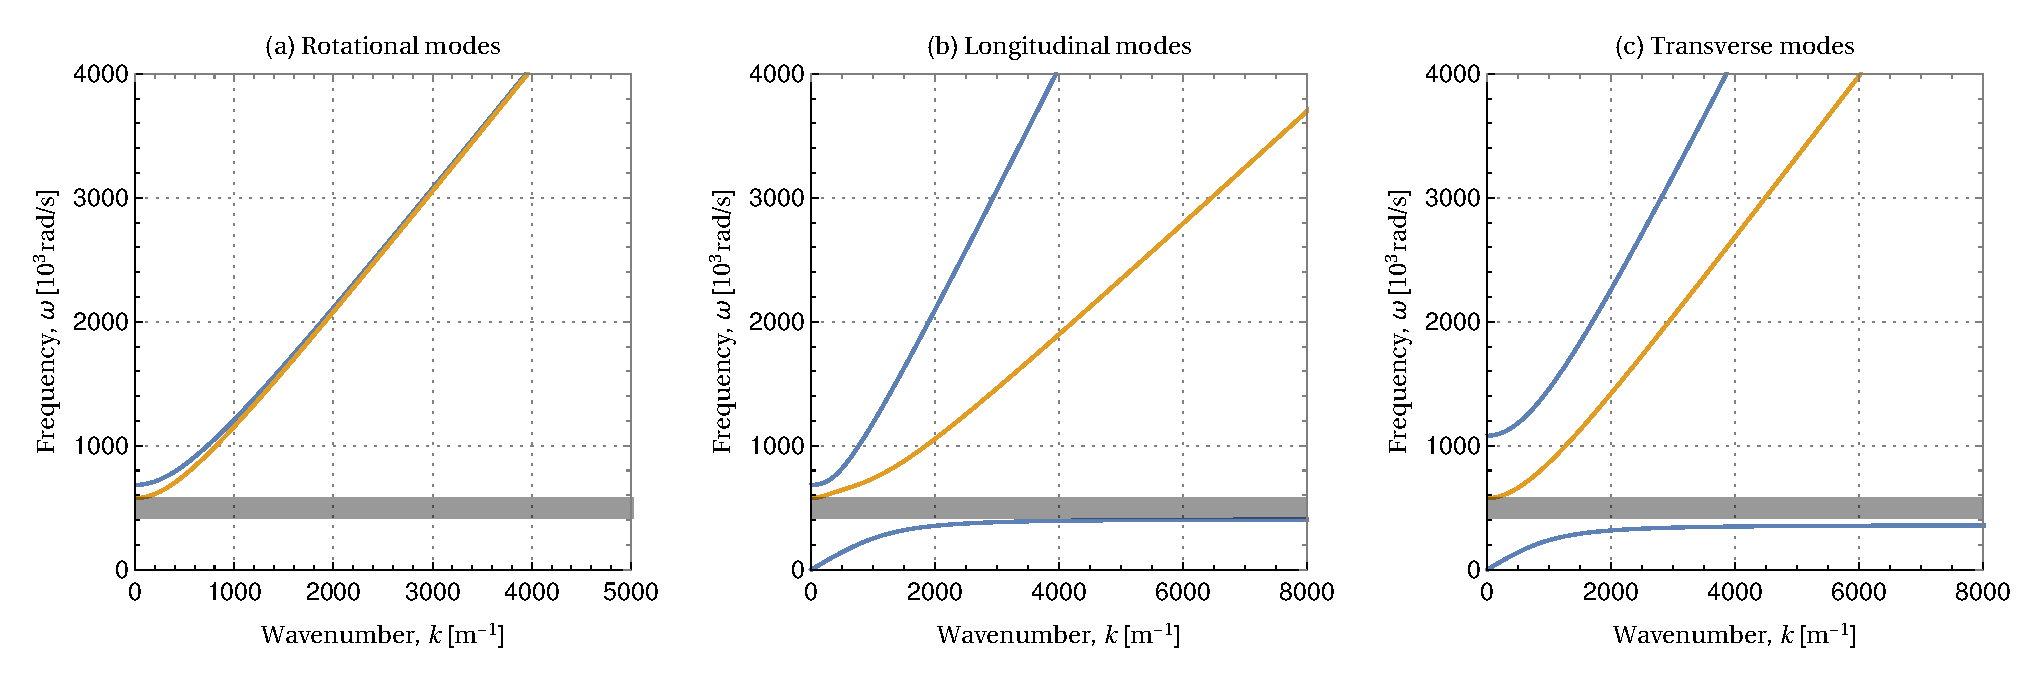
\includegraphics[draft=false,width=1.25\textwidth]{band_gap_table1}
	\end{center}
	\vspace{-4mm}
	\caption{Complete band gap (gray rectangles) for $ \mu_c >0 $.}
	\label{fig.band_gap}
\end{figure}


\begin{figure}
	\begin{center}
		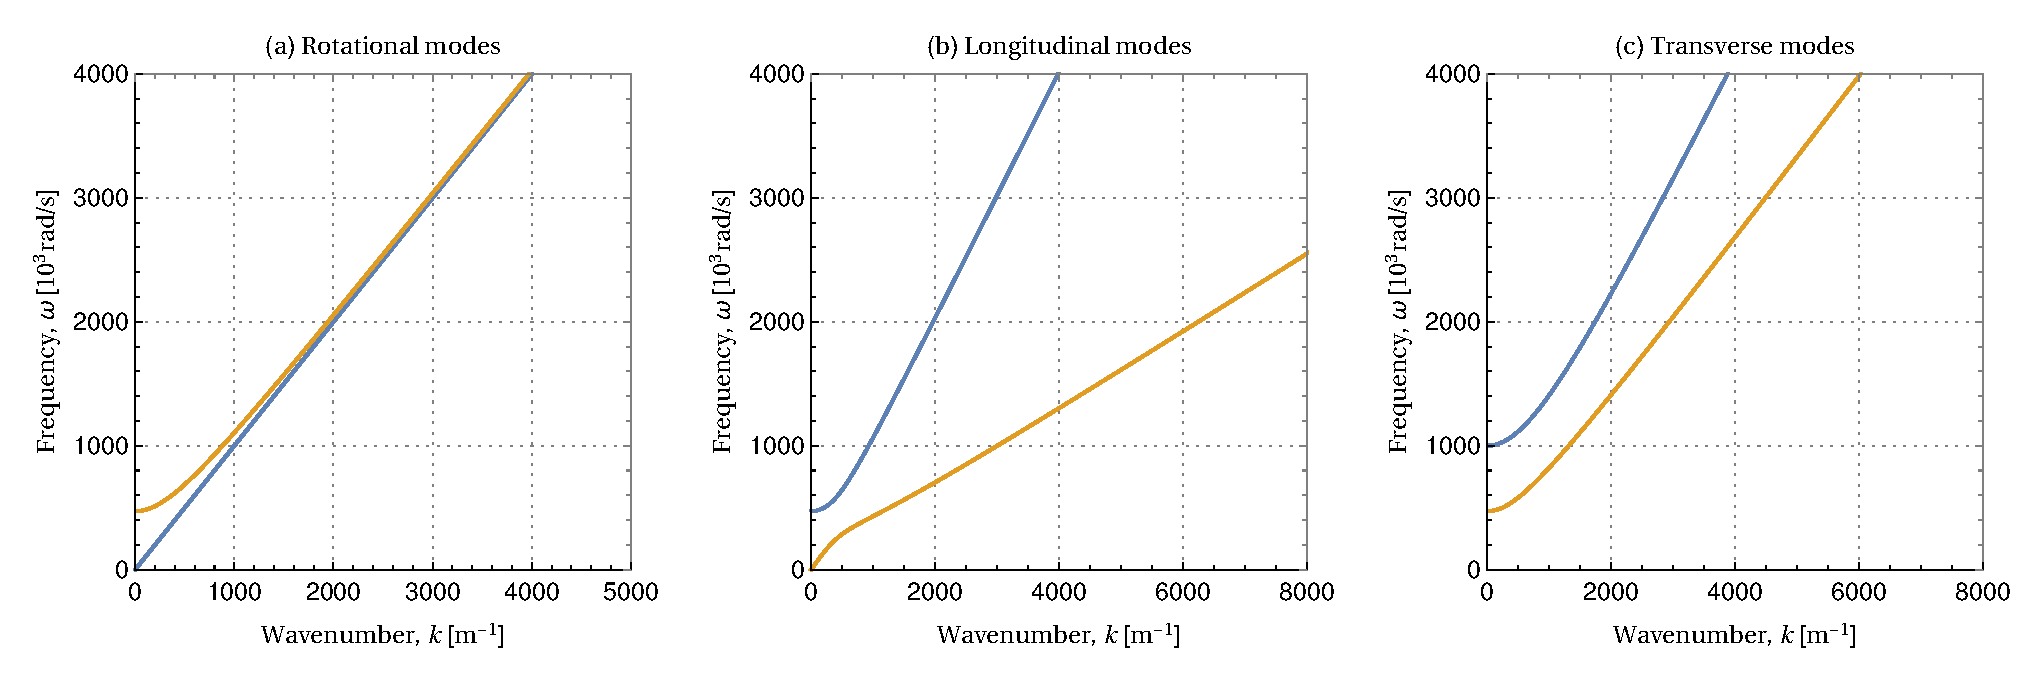
\includegraphics[draft=false,width=1.25\textwidth]{no_band_gap_table1}
	\end{center}
	\vspace{-4mm}
	\caption{No band gap for $ \mu_c = 0$.}
	\label{fig.no_band_gap}
\end{figure}

\printbibliography

\end{document}
